\documentclass[
]{jss}

\usepackage[utf8]{inputenc}

\providecommand{\tightlist}{%
  \setlength{\itemsep}{0pt}\setlength{\parskip}{0pt}}

\author{
Alfred G. Schissler\\University of Nevada \And Edward J.
Bedrick\\University of Arizona \And Alexander D. Knudson\\University of
Nevada \AND Tomasz J. Kozubowski\\University of Nevada \And Tin
Nguyen\\University of Nevada \And Anna K. Panorska\\University of Nevada
\AND Juli Petereit\\University of Nevada \And Walter W.
Piegorsch\\University of Arizona \And Duc Tran\\University of Nevada
}
\title{Simulating High-Dimensional Multivariate Data using the
\pkg{bigsimr} Package}

\Plainauthor{Alfred G. Schissler, Edward J. Bedrick, Alexander D.
Knudson, Tomasz J. Kozubowski, Tin Nguyen, Anna K. Panorska, Juli
Petereit, Walter W. Piegorsch, Duc Tran}
\Plaintitle{Simulating High-Dimensional Multivariate Data using the
bigsimr Package}
\Shorttitle{\pkg{bigsimr}: Simulate High-Dimensional Data}

\Abstract{
It is critical to accurately simulate data when employing Monte Carlo
techniques and evaluating statistical methodology. Measurements are
often correlated and high dimensional in this era of big data, such as
data obtained through high-throughput biomedical experiments. Due to
computational complexity and a lack of user-friendly software available
to simulate these massive multivariate constructions, researchers resort
to simulation designs that posit independence or perform arbitrary data
transformations. To meet this gap, we developed the bigsimr R package
for high-dimensional random vector simulation with arbitrary marginal
distributions and known Pearson, Spearman, or Kendall correlation
matrix. bigsimr contains additional high-performance features, including
multi-core algorithms to estimate correlation and compute the nearest
correlation matrix. Monte Carlo studies quantify the accuracy and
scalability of our approach, up to \(d=10,000\). Finally, we describe
example workflows and apply to a motivating high-dimensional data set
--- RNA-sequencing data obtained from breast cancer tumor samples.
}

\Keywords{multivariate simulation, high-dimensional data, nonparametric
correlation, Gaussian copula, RNA-sequencing data, breast cancer}
\Plainkeywords{multivariate simulation, high-dimensional
data, nonparametric correlation, Gaussian copula, RNA-sequencing
data, breast cancer}

%% publication information
%% \Volume{50}
%% \Issue{9}
%% \Month{June}
%% \Year{2012}
%% \Submitdate{}
%% \Acceptdate{2012-06-04}

\Address{
    Alfred G. Schissler\\
    University of Nevada\\
    1664 N Virginia St.\\
Reno, NV 89557\\
  E-mail: \email{aschissler@unr.edu}\\
  
                  }

% Pandoc citation processing

% Pandoc header

\usepackage{amsmath} \usepackage{amssymb} \usepackage{amsfonts} \usepackage{amsthm} \newtheorem{theorem}{Theorem} \newtheorem{lemma}[theorem]{Lemma} \usepackage{booktabs} \usepackage{longtable} \usepackage{array} \usepackage{ragged2e} \usepackage{setspace}

\begin{document}

\newpage

\setstretch{2.0}

\hypertarget{introduction}{%
\section{Introduction}\label{introduction}}

Massive high-dimensional (HD) data sets are now commonplace in many
areas of scientific inquiry. As new methods are developed for data
analysis, a fundamental challenge lies in designing and conducting
simulation studies to assess the operating characteristics of proposed
methodology --- such as false positive rates, statistical power,
interval coverage, and robustness --- often to compare to methods.
Further, efficient simulation empowers statistical computing strategies,
such as the parametric bootstrap \citep{Chernick2008} to simulate from a
hypothesized null model, providing inference in analytically challenging
settings. Such Monte Carlo (MC) techniques become difficult for HD
dependent data using existing algorithms and tools. This is particularly
true when simulating massive multivariate, non-normal distributions,
arising in many fields of study.

As many have noted, it can be vexing to simulate dependent,
non-normal/discrete data, even for low-dimensional (LD) settings
\citep{MB13, XZ19}. For continuous non-normal LD multivariate data, the
well-known NORmal To Anything (NORTA) algorithm \citep{Cario1997} and
other copula approaches \citep{Nelsen2007} are well-studied, with
flexible, robust software available \citep{Yan2007, Chen2001}. Yet these
approaches do not scale in a timely fashion to HD problems
\citep{Li2019gpu}. For discrete data, early simulation strategies had
major flaws, such as failing to obtain the full range of possible
correlations (e.g., admitting only positive correlations: see
\citet{Park1996}). While more recent approaches
\citep{MB13, Xia17, BF17} have largely remedied this issue for LD
problems, the existing tools are not designed to scale to high
dimensions for discrete marginal distributions.

Another central issue lies in characterizing dependence between
components in the HD random vector. The choice of correlation in
practice usually relates to the eventual analytic goal and
distributional assumptions of the data (e.g., non-normal, discrete,
infinite support, etc). For normal data, the Pearson product-moment
correlation describes the dependency perfectly. As we will see, however,
simulating arbitrary random vectors that match a target Pearson
correlation matrix is computationally intense \citep{Chen2001, Xia17}.
On the other hand, an analyst might consider use of nonparametric
correlation measures to better characterize monotone, non-linear
dependence, such as Spearman's \(\rho\) and Kendall's \(\tau\).
Throughout, we focus on matching these nonparametric dependence
measures, as our aim lies in modeling non-normal data and these
rank-based measures possess invariance properties favorable in our
proposed methodology. We do, however, implement Pearson matching, but
several layers of approximation is required.

With all this in mind, we present a scalable, flexible multivariate
simulation algorithm. The crux of the method lies in the construction of
a Gaussian copula in the spirit of the NORTA procedure. As we will
describe in more detail, the algorithm's design leverages useful
properties of nonparametric correlation measures, namely invariance
under monotone transformation and well-known closed-form relationships
between dependence measures for the multivariate normal (MVN)
distribution. For our method, we developed a high-performance
implementation: the \texttt{bigsimr} R package, written in native Julia
code.

Our study proceeds by providing background information, including a
description of a motivating example application: RNA-sequencing
(RNA-seq) breast cancer data. Then we describe and justify our
simulation methodology and related algorithms. We proceed by providing
an illustrative LD \texttt{bigsimr} workflow. Next we conduct MC studies
under various bivariate distributional assumptions to evaluate
performance and accuracy. After the MC evaluations, we simulate random
vectors motivated by our RNA-seq example, evaluate the accuracy, and
provide example statistical computing tasks, namely MC estimation of
joint probabilities and evaluating HD correlation estimation efficiency.
Finally, we discuss the method's utility, limitations, and future
directions.

\hypertarget{background}{%
\section{Background}\label{background}}

The \texttt{bigsimr} \texttt{R} package presented here provides multiple
algorithms that operate with HD multivariate data; however, all these
algorithms were originally designed to support a single task: to
generate random vectors drawn from multivariate probability
distributions with given marginal distributions and dependency metrics.
Specifically, our goal is to efficiently simulate a large number, \(B\),
of HD random vectors \({\bf Y}=(Y_1, \ldots, Y_d)^\top\) with
\emph{correlated} components and heterogeneous marginal distributions,
described via cumulative distribution functions (CDFs)
\(F_i, i=1,\ldots,d\).

When designing this methodology, we developed the following properties
to guide our effort. We divide the properties into two categories: (1)
basic properties (BP) and ``scalability'' properties (SP). The BPs are
adapted from an existing criteria due to \citet{Nik13a}. A suitable
simulation strategy should possess the following properties:

\setstretch{1.5}

\begin{itemize}
\tightlist
\item
  BP1: A wide range of dependences, allowing both positive and negative
  values, and, ideally, admitting the full range of possible values.
\item
  BP2: Flexible dependence, meaning that the number of bivariate
  marginals can be equal to the number of dependence parameters.
\item
  BP3: Flexible marginal modeling, generating heterogeneous data ---
  including mixed continuous and discrete margins.
\end{itemize}

\setstretch{2.0}

Moreover, the simulation method must \emph{scale} to high dimensions:

\setstretch{1.5}

\begin{itemize}
\tightlist
\item
  SP1: Procedure must scale to high dimensions with practical compute
  times.
\item
  SP2: Procedure must scale to high dimensions while maintaining
  accuracy.
\end{itemize}

\setstretch{2.0}

\hypertarget{motivating-example-rna-seq-data}{%
\subsection{Motivating example: RNA-seq
data}\label{motivating-example-rna-seq-data}}

Simulating HD, non-normal, correlated data motivates this work, in
pursuit of modeling RNA-sequencing (RNA-seq) data
\citep{Wang2009b, Conesa2016b} derived from breast cancer patients. The
RNA-seq data-generating process involves counting how often a particular
form of messenger RNA (mRNA) is expressed in a biological sample.
RNA-seq platforms typically quantify the entire transcriptome in one
experimental run, resulting in HD data. For human-derived samples, this
results in count data corresponding to over 20,000 genes (protein-coding
genomic regions) or even over 77,000 isoforms when alternatively-spliced
mRNA are counted \citep{Schissler2019}. Importantly, due to inherent
biological processes, gene expression data exhibit correlation
(co-expression) across genes \citep{BE07, Schissler2018}.

We illustrate our methodology using the Breast Invasive Carcinoma (BRCA)
data set housed in The Cancer Genome Atlas (TCGA; see Acknowledgments).
For ease of modeling and simplicity of exposition, we only consider high
expressing genes. In turn, we begin by filtering to retain the top 1000
of the highest-expressing genes (in terms of median expression) of the
over 20,000 gene measurements from \(N=878\) patients' tumor samples.
This gives a great number of pairwise dependencies among the marginals
(specifically, \(\ensuremath{4.995\times 10^{5}}\) correlation
parameters). Table @ref(tab:ch010-realDataTab) displays RNA-seq counts
for three selected high-expressing genes for the first five patients'
breast tumor samples. To help visualize the bivariate relationships for
these three selected genes across all patients, Figure
@ref(fig:ch010-realDataFig) displays the marginal distributions and
estimated Spearman's correlations.

\begin{CodeChunk}
\begin{table}

\caption{\label{tab:ch010-realDataTab}mRNA expression for three selected high-expressing genes, STAU1, FKBP1A, NME2, for the first five patients in the TCGA BRCA data set.}
\centering
\begin{tabular}[t]{lrrr}
\toprule
Patient ID & STAU1 & FKBP1A & NME2\\
\midrule
TCGA-A1-A0SB & 10440 & 11354 & 17655\\
TCGA-A1-A0SD & 21523 & 20221 & 14653\\
TCGA-A1-A0SE & 21733 & 22937 & 35251\\
TCGA-A1-A0SF & 11866 & 19650 & 16551\\
TCGA-A1-A0SG & 12486 & 12089 & 10434\\
\bottomrule
\end{tabular}
\end{table}

\end{CodeChunk}

\begin{CodeChunk}
\begin{figure}

{\centering 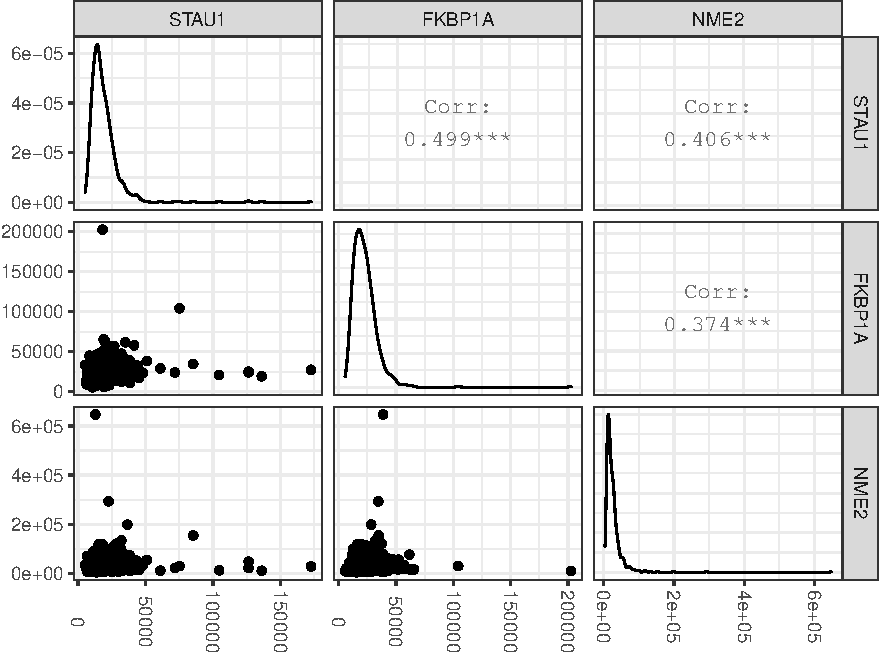
\includegraphics[width=0.85\linewidth]{article_bigsimr_files/figure-latex/ch010-realDataFig-1} 

}

\caption[Pairwise scatterplots for three example genes (Table 1), with estimated Spearman's correlations and marginal density estimates displayed]{Pairwise scatterplots for three example genes (Table 1), with estimated Spearman's correlations and marginal density estimates displayed. The data possess outliers, heavy-right tails, are discrete, and have non-trivial intergene correlations. Modeling these data motivate our simulation methodology.}\label{fig:ch010-realDataFig}
\end{figure}
\end{CodeChunk}

\hypertarget{measures-of-dependency}{%
\subsection{Measures of dependency}\label{measures-of-dependency}}

In multivariate analysis, an analyst must select a metric to quantify
dependency. The most widely-known is the Pearson correlation coefficient
that describes the linear association between two random variables \(X\)
and \(Y\), and, it is given by

\begin{equation}
\rho_P(X,Y) = \frac{E(XY) - E(X)E(Y)}{\left[ \mathrm{Var}(X)\mathrm{Var}(Y)\right]^{1/2}}.
\label{eq:pearson}
\end{equation}

As \citet{MB13} and \citet{MK01} discuss, for a bivariate normal
\((X,Y)\) random vector, the Pearson correlation completely describes
the dependency between the components. For non-normal marginals with
monotone correlation patterns, however, \(\rho_P\) suffers some
drawbacks and may mislead or fail to capture important relationships
\citep{MK01}. Alternatively, analysts often prefer rank-based
correlation measures to describe the degree of monotonic association.

Two nonparametric, rank-based measures common in practice are Spearman's
correlation (denoted \(\rho_S\)) and Kendall's \(\tau\). Spearman's
\(\rho_S\) has an appealing correspondence as the Pearson correlation
coefficient on \emph{ranks} of the values, thereby capturing nonlinear
yet monotone relationships. Kendall's \(\tau\), on the other hand, is
the difference in probabilities of concordant and discordant pairs of
observations, \((X_i, Y_i)\) and \((X_j, Y_j)\) (concordance meaning
that orderings have the same direction, e.g., if \(X_i < X_j\), then
\(Y_i < Y_j\)). Note that concordance is determined by the ranks of the
values, not the values themselves.

Both \(\tau\) and \(\rho_S\) are \emph{invariant under monotone
transformations} of the underlying random variates. As we will describe
more fully in the \protect\hyperlink{algorithms}{Algorithms} section,
this property enables matching rank-based correlations with speed (SP1)
and accuracy (SP2).

\emph{Correspondence among Pearson, Spearman, and Kendall correlations}

There is no closed form, general correspondence among the rank-based
measures and the Pearson correlation coefficient, as the marginal
distributions \(F_i\) are intrinsic in their calculation. For
\emph{bivariate normal vectors}, however, the correspondence is
well-known:

\begin{equation}
\label{eq:convertKendall}
\rho_{P} = \sin \left( \tau \times \frac{\pi}{2} \right), 
\end{equation}

\noindent and similarly for Spearman's \(\rho\) \citep{K58},

\begin{equation}
\label{eq:convertSpearman}
\rho_P = 2 \times \sin \left( \rho_S \times \frac{\pi}{6} \right).
\end{equation}

\emph{Marginal-dependent bivariate correlation bounds}

Given two marginal distributions, \(\rho_P\) is not free to vary over
the entire range of possible correlations \([-1,1]\). The
\emph{Frechet-Hoeffding bounds} are well-studied
\citep{Nelsen2007, BF17}. These constraints cannot be overcome through
algorithm design. In general, the bounds are given by

\begin{equation}
\label{eq:frechet}
\rho_P^{max} = \rho_P \left( F^{-1}_1 (U), F^{-1}_2 (U) \right), \quad \rho_P^{min} = \rho_P \left( F^{-1}_1 (U), F^{-1}_2 (1 - U) \right)
\end{equation}

\noindent where \(U\) is a uniform random variable on \((0,1)\) and
\(F^{-1}_1, F^{-1}_2\) are the inverse CDFs of \(X_1\) and \(X_2\),
respectively, definitely by @ref(eq:inverseCDF) when the variables are
discrete.

\begin{equation}
F_{i}^{-1} = \inf\{y:F_{i}(y) \geq u \}.
\label{eq:inverseCDF}
\end{equation}

\hypertarget{gaussian-copulas}{%
\subsection{Gaussian copulas}\label{gaussian-copulas}}

There is a connection of our simulation strategy to Gaussian
\emph{copulas} \citep{Nelsen2007}. A copula is a distribution function
on \([0,1]^d\) that describes a multivariate probability distribution
with standard uniform marginals. This provides a powerful, natural way
to characterize joint probability. Consequently, the study of copulas is
an important and active area of statistical theory and practice.

For any random vector \({\bf X}=(X_1, \ldots, X_d)^\top\) with CDF \(F\)
and marginal CDFs \(F_i\) there is a copula function
\(C(u_1, \ldots, u_d)\) satisfying

\begin{equation}
F(x_1, \ldots, x_d) = {\mathbb P}(X_1\leq x_1, \ldots,X_d\leq x_d) = C(F_1(x_1), \ldots, F_d(x_d)), 
\label{eq:copula}
\end{equation}

\(x_i \in {\mathbb R}, i=1,\ldots,d.\)

A Gaussian copula has marginal CDFs that are all standard normal,
\(F_i = \Phi, \forall \, i\), where \(\Phi(\cdot)\) is the standard
normal CDF. This representation corresponds to a multivariate normal
(MVN) distribution with standard normal marginal distributions and
covariance matrix \({\bf R_P}\). Since the marginals are standardized to
have unit variance, however, \({\bf R_P}\) is a Pearson correlation
matrix. If \(F_{{\bf R}}\) is the CDF of such a multivariate normal
distribution, then the corresponding Gaussian copula \(C_{{\bf R}}\) is
defined through

\begin{equation}
\label{eq:gauss}
F_{{\bf R}}(x_1, \ldots, x_d) = C_{{\bf R}}(\Phi(x_1), \ldots, \Phi(x_d)),
\end{equation}

Here the copula function \(C_{{\bf R}}\) is the familiar multivariate
normal CDF of the random vector \((\Phi(X_1), \ldots, \Phi(X_d))\),
where \((X_1, \ldots, X_d) \sim N_d({\bf 0}, {\bf R_P})\).

Sklar's Theorem \citep{Sklar1959, Ubeda-Flores2017} guarantees that
given inverse CDFs \(F_i^{-1}\)s and a valid correlation matrix (within
the Frechet bounds) a random vector can be obtained via transformations
involving copula functions. For example, using Gaussian copulas, we can
construct a random vector \({\bf Y} = (Y_1, \ldots, Y_d)^\top\) with
\(Y_i \sim F_i\), viz.~\(Y_i = F_i^{-1}(\Phi(X_i)), i=1, \ldots, d\),
where \((X_1, \ldots, X_d) \sim N_d({\bf 0}, {\bf R_P})\).

\hypertarget{other-multivariate-simulation-r-packages}{%
\subsection{Other Multivariate Simulation R
Packages}\label{other-multivariate-simulation-r-packages}}

To place \texttt{bigsimr}'s implementation and algorithms in context
with existing approaches, here we qualitatively compare to other
\texttt{R} multivariate simulation packages. The \texttt{MASS} packages
\texttt{mvnorm()} has long been available to produce random vectors from
multivariate normal (and \(t\)) distributions. This familiar procedure
cannot simulate from arbitrary margins and dependency measures, as well
as fails to readily scale to high dimensions. Recently, the
high-performance package \texttt{mvnfast} \citep{Fasiolo2016} has been
released that provides HD multivariate normal generation, but this lacks
flexibility in marginal models and dependency modeling. For dependent
discrete data, LD packages exist, such as \texttt{GenOrd}. For copula
computation, the full-featured package \texttt{copula} provides many
different copulas and a fairly general LD random generator
\texttt{rCopula()}. High-dimesional random vectors via \texttt{copula}
takes an impractical amount of computing time \citep{Li2019gpu}. The
\texttt{nortaRA} R package matches Pearson coefficients near exactly and
is reasonable for LD settings. Finally, we know of no other \texttt{R}
package that can produce HD random vectors with flexible margins and
dependence modeling. Table (\#tab:compare-table) summarizes the above
discussion.

\begin{table}[]
\centering
\caption{Selected feature comparison of bigsimr to existing R packages for multivariate simulation.}
\label{tab:compare-table}
\begin{tabular}{@{}llll@{}}
R Package & Scales to HD & Hetereogenous Margins & Flexible Dependence \\ \midrule
MASS      & No           & No                    & No                  \\
mvnfast   & Yes          & No                    & No                  \\
GenOrd    & No           & Discrete margins      & Yes                 \\
copula    & No           & Yes                   & No                  \\
nortaRA   & No           & Yes                   & No                  \\
bigsimr   & Yes          & Yes                   & Yes                
\end{tabular}
\end{table}

\hypertarget{algorithms}{%
\section{Algorithms}\label{algorithms}}

This section describes our methods involved in simulating a random
vector \(\bf Y\) with \(Y_i\) components for \(i=1,\ldots,d\). Each
\(Y_i\) has a specified marginal CDF \(F_i\) and its inverse
\(F^{-1}_i\). To characterize dependency, every pair \((Y_i, Y_j)\) has
a given Pearson correlation \(\rho_P\), Spearman correlation \(\rho_S\),
and/or Kendall's \(\tau\). The method can be described as a
\emph{high-performance Gaussian copula} (Equation @ref(eq:gauss))
providing a HD NORTA-inspired algorithm.

\hypertarget{normal-to-anything-norta}{%
\subsection{NORmal To Anything (NORTA)}\label{normal-to-anything-norta}}

The well-known NORTA algorithm \citep{Cario1997} simulates a random
vector \(\bf Y\) with variance-covariance matrix \(\Sigma_{\bf Y}\).
Specifically, NORTA algorithm proceeds as:

\setstretch{1.5}

\begin{enumerate}
\def\labelenumi{\arabic{enumi}.}
\tightlist
\item
  Simulate a random vector \(\bf Z\) with \(d\) independent and
  identically distributed (iid) standard normal components.
\item
  Determine the input matrix \(\Sigma_{\bf Z}\) that corresponds with
  the specified output \(\Sigma_{\bf Y}\).
\item
  Produce a Cholesky factor \(M\) of \(\Sigma_{\bf Z}\) such that
  \(M M^{\prime}=\Sigma_{\bf Z}\).
\item
  Set \(X\) by \(X \gets MZ\).
\item
  \(\text{Return} \; Y \; \text{where} \; Y_i \gets F_i^{-1}[\Phi(X_i)], \; i=1,...,d\).
\end{enumerate}

\setstretch{2.0}

With modern parallel computing, steps 1, 3, 4, 5 are readily implemented
as high-performance, multi-core and/or graphical-processing-unit (GPU)
accelerated algorithms --- providing fast scalability to HD.

Matching specified Pearson correlation coefficients exactly (step 2
above), however, is computationally costly. In general, there is no
convenient correspondence between the components of the input
\(\Sigma_{\bf Z}\) and target \(\Sigma_{\bf Y}\). Matching the
correlations involves evaluating or approximating \(\binom{d}{2}\)
integrals of the form

\begin{equation}
    \mathrm{E}\left[Y_i Y_j\right] = \int_{-\infty}^{\infty} \int_{-\infty}^{\infty} F_i^{-1}\left[\Phi(z_i)\right] F_j^{-1}\left[\Phi(z_j)\right] \phi(z_i, z_j, \rho_z) dz_i dz_j,
    \label{eq:pearsonIntegralRelation}
\end{equation}

where \(\phi(\cdot)\) is the joint probability distribution function of
two correlated standard normal variables. For HD simulation, exact
evaluation may become too costly to enable practical simulation studies.
Our remedy to enable HD Pearson matching in \texttt{bigsimr} is Hermite
polynomial approximation of these \(\choose{d}{2}\) double integrals, as
suggested by \citet{XZ19}.

\emph{NORTA in higher dimensions}

Sklar's theorem provides a useful characterization of multivariate
distributions through copulas. Yet the choice of copula-based simulation
algorithm affects which joint distributions may be simulated. Even in LD
spaces (e.g., \(d=3\)), there exist valid multivariate distributions
with \emph{feasible} Pearson correlation matrices that NORTA cannot
match exactly \citep{LH75}. This occurs when the bivariate
transformations are applied to find the input correlation matrix, yet
when combined the resultant matrix is indefinite. These situations do
occur, even using exact analytic calculations. Such problematic target
correlation matrices are termed \emph{NORTA defective}.

\citet{GH02} conducted a Monte Carlo study to estimate the probability
of encountering NORTA defective matrices while increasing the dimension
\(d\). They found that for what is now considered low-to-moderate
dimensions (\(d \approx 20\)), almost \emph{all} feasible matrices are
NORTA defective. This stems from the concentration of measure near the
boundary of the space of all possible correlation matrices as dimension
increases. Unfortunately, it is precisely near this boundary that NORTA
defective matrices reside.

There is hope, however, as \citet{GH02} also showed that replacing an
indefinite input correlation matrix with a close proxy will give
approximate matching to the target --- with adequate performance for
moderate \(d\). This provides guidance that our nearest positive
definite (PD) augmented approach has promise provide adequate accuracy
if our input matching scheme returns an indefinite matrix.

\hypertarget{rand-vec-gen}{%
\subsection{bigsimr rvec: Random vector generator}\label{rand-vec-gen}}

We now describe our algorithm to generate random vectors, which extends
NORTA to HD via nearest correlation matrix replacement and provides
rank-based dependency matching:

\setstretch{1.5}

\begin{enumerate}
\def\labelenumi{\arabic{enumi}.}
\tightlist
\item
  Mapping step, either

  \begin{itemize}
  \tightlist
  \item
    Convert the target Spearman correlation matrix \(R_S\) to the
    corresponding MVN Pearson correlation \(R_X\). Alternatively,
  \item
    Convert the target Kendall \(\tau\) matrix \(R_K\) to the
    corresponding MVN Pearson correlation \(R_X\). Alternatively,
  \item
    Convert the target Pearson correlation matrix to \(R_P\) to the
    corresponding, approximate MVN Pearson correlation \(R_X\).
  \end{itemize}
\item
  Check admissibility and, if needed, compute the nearest correlation
  matrix.

  \begin{itemize}
  \tightlist
  \item
    Check that \(R_X\) is a correlation matrix, a positive definite
    matrix with 1's along the diagonal.
  \item
    If \(R_X\) is a correlation matrix, the input matrix is
    \emph{admissible} in this scheme. Otherwise,
  \item
    Replace \(R_X\) with the nearest correlation matrix \(\tilde{R}_X\),
    in the Frobenius norm.
  \end{itemize}
\item
  Gaussian copula

  \begin{itemize}
  \tightlist
  \item
    Generate \({\bf X}=(X_1, \ldots, X_d) \sim N_d({\bf 0}, R_X)\).
  \item
    Transform \({\bf X}\) to \({\bf U} = (U_1, \ldots, U_d)\)
    viz.~\(U_i=\Phi(X_i)\), \(i=1, \ldots, d\).
  \item
    Return \({\bf Y} = (Y_1, \ldots, Y_d)\), where
    \(Y_i=F_i^{-1}(U_i)\), \(i=1, \ldots, d\).
  \end{itemize}
\end{enumerate}

\emph{Step 1: Mapping step.} We first employ the closed-form
relationships between \(\rho_S\) and \(\tau\) with \(\rho_P\) for
bivariate normal random variables via Equations @ref(eq:convertKendall)
and @ref(eq:convertSpearman), respectively (implemented as
\texttt{cor\_covert()}). Initializing our algorithm to match the
nonparametric correlations by computing these equations for all pairs is
computationally trivial.

For the computationally expensive process to match Pearson correlations,
we approximate Equation @ref(eq:pearsonIntegralRelation) for all pairs
of margins. To this end, we implement the approximation scheme
introduced by \citet{xiao2019matching}. Briefly, the many double
integrals of the form in @ref(eq:pearsonIntegralRelation) are
approximated by weighted sums of Hermite polynomials. Matching
coefficients for pairs of continuous distributions is made tractable by
this method, but for discrete distributions (especially discrete
distributions with large support sets or infinite support), the
approximation is computationally expensive. To remedy this, we further
approximate discrete distributions by a continuous distribution using
Generalized S-Distributions \citep{muino2006gs}.

\emph{Step 2: Admissibility check and nearest correlation matrix
computation.} Once \(R_X\) has been determined, we check admissibility
of the adjusted correlation via the steps described above. If \(R_X\) is
not a valid correlation matrix, then we compute the nearest correlation
matrix. Finding the nearest correlation matrix is a common statistical
computing problem. The defacto function in \texttt{R} is
\texttt{Matrix::nearPD}, an alternating projection algorithm due to
\citet{higham2002computing}. As implemented the function fails to scale
to HD. Instead, we provide the quadratically-convergent algorithm based
on the theory of strongly semi-smooth matrix functions
(\citet{qi2006quadratically}). The nearest correlation matrix problem
can be written down as the following convex optimization problem:
\(\mathrm{min} \quad \frac{1}{2} \Vert G - X \Vert^2, \quad \mathrm{s.t.} \quad X_{ii} = 1, \quad i = 1, \ldots , n, \quad X \in S_{+}^{n}\).

For nonparametric correlation measures, our algorithm allows the
generation of HD multivariate data with arbitrary marginal distributions
with a broad class of admissible Spearman correlation matrices and
Kendall \(\tau\) matrices. The admissible classes consist of the
matrices that map to a Pearson correlation matrix for a MVN. In
particular, if we let \(X\) be MVN with \(d\) components and denote
\(\Omega_P = \{ R_P : R_P \textrm{ is a correlation matrix for } X \}, \quad \Omega_K = \{ R_K : R_K \textrm{ is a correlation matrix for } X \}, \quad \Omega_S = \{ R_S : R_S \textrm{ is a correlation matrix for } X \}\).
There are 1-1 mappings between these sets. We conjecture that the sets
of admissible \(R_S\) and \(R_K\) are not highly restrictive. In
particular, \(R_P\) is approximately \(R_S\) for a MVN, suggesting that
the admissible set \(\Omega_S\) should be flexible as \(R_P\) can be any
PD matrix with 1's along the diagonal. We provide methods to check
whether a target \(R_S\) is an element of the \emph{admissible set}
\(\Omega_S\).

There is an increasing probability of encountering a inadmissible
correlation matrix as dimension increases. In our experience, the
mapping step for large \(d\) almost always produces a \(R_X\) that is
not a correlation matrix. In Section @ref(package) we provide a basic
description of how to quantify and control the approximation error.
Further, the RNA-seq example in Section @ref(examples) provides an
illustration of this in practice.

\emph{Step 3: Gaussian copula.} The final step implements a
NORTA-inspired, Gaussian copula approach to produce the desired margins.
Steps 1 and 2 determine the MVN Pearson correlation values that will
eventually match the target correlation. Step 3 requires a fast MVN
simulator, a standard normal CDF, and well-defined quantile functions
for marginals. The MVN is transformed to a copula (distribution with
standard uniform margins) by applying the normal CDF \(\Phi(\cdot)\).
Finally, the quantile functions \(F^{-1}\) are applied across the
margins to return the desired random vector \({\bf Y}\).

\section[bigsimr-pkg]{The \pkg{bigsimr} R package}\label{package}

This section describes a LD random vector simulation workflow via the
\texttt{bigsimr} \texttt{R} package. Our \texttt{R} package provides an
interface to the native code written in Julia (registered as the
\texttt{Bigsimr} Julia package. In addition to the native Julia
\texttt{Bigsimr} package and \texttt{R} interface \texttt{bigsimr}, we
also provide a python interface \texttt{bigsimr} that interfaces with
the Julia \texttt{Bigsimr} package. The Julia package provides a
high-performance implementation of our proposed random vector generation
algorithm and associated functions (see Section @ref(algorithms)).

The subsections below describe the basic use of \texttt{bigsimr} by
stepping through an example workflow using the data set
\texttt{airquality} that contains daily air quality measurements in New
York, May to September 1973 \citep{Chambers1983}. This workflow proceeds
from setting up the computing environment, to data wrangling,
estimation, simulation configuration, random vector generation, and,
finally, result visualization.

\hypertarget{bivariate-example}{%
\subsection{Bivariate example}\label{bivariate-example}}

We illustrate the use of \texttt{bigsimr} using the New York air quality
data set (\texttt{airquality}) included in the R \texttt{datasets}
package. First, we load the \texttt{bigsimr} library and a few other
convenient data science packages, including the syntactically-elegant
\texttt{tidyverse} suite of \texttt{R} packages. The code chunk below
prepares the computing environment:

\begin{CodeChunk}
\begin{CodeInput}
R> library("tidyverse")
R> library("bigsimr")
R> # Activate multithreading in Julia
R> Sys.setenv(JULIA_NUM_THREADS = parallel::detectCores())
R> # Load the Bigsimr and Distributions Julia packages
R> bs <- bigsimr_setup()
R> dist <- distributions_setup()
\end{CodeInput}
\end{CodeChunk}

Below, we describe a minimal working example --- a bivariate simulation
of two airquality variables: \texttt{Temperature}, in degrees
Fahrenheit, and \texttt{Ozone} level, in parts per billion.

\begin{CodeChunk}
\begin{CodeInput}
R> df <- airquality %>% select(Temp, Ozone) %>% drop_na()
\end{CodeInput}
\end{CodeChunk}

\begin{CodeChunk}
\begin{CodeOutput}
Rows: 116
Columns: 2
$ Temp  <int> 67, 72, 74, 62, 66, 65, 59, 61, 74, 69, 66, 68, 58, 64, 66, 57, ~
$ Ozone <int> 41, 36, 12, 18, 28, 23, 19, 8, 7, 16, 11, 14, 18, 14, 34, 6, 30,~
\end{CodeOutput}
\end{CodeChunk}

Figure @ref(fig:ch030-aq-joint-dist) visualizes the bivariate
relationship between \texttt{Ozone} and \texttt{Temperature}. We aim to
simulate random two-component vectors mimicking this structure. The
margins are not normally distributed; \texttt{Ozone} level exhibits a
strong positive skew.

\begin{CodeChunk}
\begin{figure}

{\centering 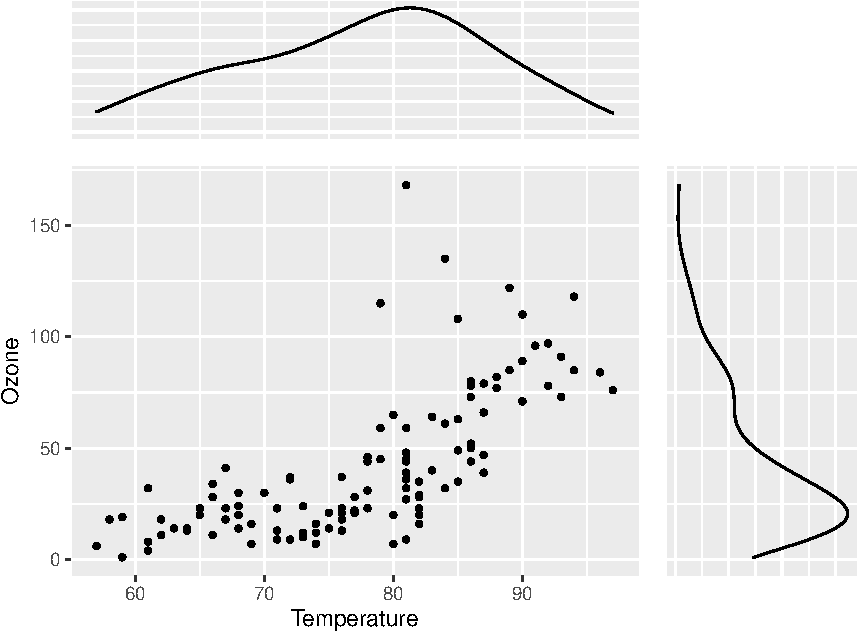
\includegraphics[width=0.85\linewidth]{article_bigsimr_files/figure-latex/ch030-aq-joint-dist-1} 

}

\caption[Bivariate scatterplot of Ozone versus Temp with estimated marginal densities]{Bivariate scatterplot of Ozone versus Temp with estimated marginal densities. The Ozone data are modeled marginally as log-normal and the Temperature data as normal.}\label{fig:ch030-aq-joint-dist}
\end{figure}
\end{CodeChunk}

Next, we specify the marginal distributions and correlation coefficient
(both type and magnitude). Here the analyst is free to be creative. For
this example, we avoid goodness-of-fit considerations to determine the
marginal distributions. It is sensible without domain knowledge to
estimate these quantities from the data, and \texttt{bigsimr} contains
fast functions designed for this task.

\hypertarget{specifying-marginal-distributions}{%
\subsection{Specifying marginal
distributions}\label{specifying-marginal-distributions}}

Based on the estimated densities in Figure
@ref(fig:ch030-aq-joint-dist), we assume \texttt{Temp} is normally
distributed and \texttt{Ozone} is log-normally distributed, as the
latter values are positive and skewed. We use the classical unbiased
estimators for the normal distribution's parameters and maximum
likelihood estimators for the log-normal parameters:

\begin{CodeChunk}
\begin{CodeInput}
R> df %>% select(Temp) %>% 
+   summarise_all(.funs = c(mean = mean, sd = sd))
\end{CodeInput}
\begin{CodeOutput}
   mean    sd
1 77.87 9.485
\end{CodeOutput}
\end{CodeChunk}

\begin{CodeChunk}
\begin{CodeInput}
R> mle_mean <- function(x) mean(log(x))
R> mle_sd <- function(x) mean( sqrt( (log(x) - mean(log(x)))^2 ) )
R> df %>% 
+   select(Ozone) %>% 
+   summarise_all(.funs = c(meanlog = mle_mean, sdlog = mle_sd))
\end{CodeInput}
\begin{CodeOutput}
  meanlog  sdlog
1   3.419 0.6967
\end{CodeOutput}
\end{CodeChunk}

Now, we configure the input marginals for later input into
\texttt{rvec}. The marginal distributions are specified using
\texttt{Julia}'s \texttt{Distributions} package and stored in a vector.

\begin{CodeChunk}
\begin{CodeInput}
R> margins <- c(dist$Normal(mean(df$Temp), sd(df$Temp)),
+              dist$LogNormal(mle_mean(df$Ozone), mle_sd(df$Ozone)))
\end{CodeInput}
\end{CodeChunk}

\hypertarget{specifying-correlation}{%
\subsection{Specifying correlation}\label{specifying-correlation}}

As mentioned, the user must decide how to describe correlation based on
the particulars of the problem. For non-normal data and for improved
simulation accuracy/scalability in our scheme, we advocate the use of
Spearman's \(\rho\) correlation matrix \(R_S\) and Kendall's \(\tau\)
correlation matrix \(R_K\). We also support Pearson correlation
coefficient matching, while cautioning the user to check the performance
for the distribution at hand (see \protect\hyperlink{simulations}{Monte
Carlo evaluations} below for evaluation strategies and guidance). Note
that hese estimation methods are classical approaches, not specifically
designed for high-dimensional correlation estimation.

\begin{CodeChunk}
\begin{CodeInput}
R> (R_S <- bs$cor(as.matrix(df), bs$Spearman))
\end{CodeInput}
\begin{CodeOutput}
      [,1]  [,2]
[1,] 1.000 0.774
[2,] 0.774 1.000
\end{CodeOutput}
\end{CodeChunk}

\hypertarget{checking-target-correlation-matrix-admissibility}{%
\subsection{Checking target correlation matrix
admissibility}\label{checking-target-correlation-matrix-admissibility}}

Once a target correlation matrix is specified, first convert the
dependency type to Pearson to correctly specify the MVN inputs. Then,
check that the converted matrix \(R_X\) is a valid correlation matrix
(PD and 1s on the diagonal). For this bivariate example, \(R_X\) is a
valid correlation matrix. Typically in HD the resultant MVN Pearson
correlation matrix is indefinite and requires approximation (see the HD
examples in subsequent sections).

\begin{CodeChunk}
\begin{CodeInput}
R> # Step 1. Mapping
R> (R_X <- bs$cor_convert(R_S, bs$Spearman, bs$Pearson))
\end{CodeInput}
\begin{CodeOutput}
       [,1]   [,2]
[1,] 1.0000 0.7886
[2,] 0.7886 1.0000
\end{CodeOutput}
\end{CodeChunk}

\begin{CodeChunk}
\begin{CodeInput}
R> # Step 2. Check admissibility
R> bs$iscorrelation(R_X)
\end{CodeInput}
\begin{CodeOutput}
[1] TRUE
\end{CodeOutput}
\end{CodeChunk}

Despite being a valid correlation matrix under this definition, marginal
distributions induce Frechet bounds on the possible Pearson correlation
values. To check that the converted correlation values fall within these
bounds, use \texttt{bigsimr::cor\_bounds} to estimate the pairwise lower
and upper correlation bounds. \texttt{cor\_bounds} uses the Generate,
Sort, and Correlate algorithm of \citet{DH2011}. For the assumed
marginals, the Pearson correlation coefficient is not free to vary in
{[}-1,1{]}, as seen below. Our MC estimate of the bounds slightly
underestimates the theoretic bounds of \((-0.881, 0.881)\). (See an
analytic derivation presented in the Appendix). Since our single Pearson
correlation coefficient is within the theoretical bounds, the
correlation matrix is valid for our simulation strategy.

\begin{CodeChunk}
\begin{CodeInput}
R> bs$cor_bounds(margins[1], margins[2], bs$Pearson, n_samples = 1e6)
\end{CodeInput}
\begin{CodeOutput}
Julia Object of type NamedTuple{(:lower, :upper),Tuple{Float64,Float64}}.
(lower = -0.8807818345178882, upper = 0.8817164736117079)
\end{CodeOutput}
\end{CodeChunk}

\hypertarget{simulating-random-vectors}{%
\subsection{Simulating random vectors}\label{simulating-random-vectors}}

A single \texttt{rvec} execution simulates the desired \(10,000\) random
vectors from the assumed bivariate distribution of \texttt{Ozone} and
\texttt{Temp}. Note that the target input in specified using the
pre-computed MVN correlation matrix.

\begin{CodeChunk}
\begin{CodeInput}
R> x <- bs$rvec(10000, R_X, margins)
R> df_sim <- as.data.frame(x)
R> colnames(df_sim) <- colnames(df)
\end{CodeInput}
\end{CodeChunk}

Figure @ref(fig:ch030-plot-sim) plots the 10,000 simulated points.

\begin{CodeChunk}
\begin{figure}

{\centering 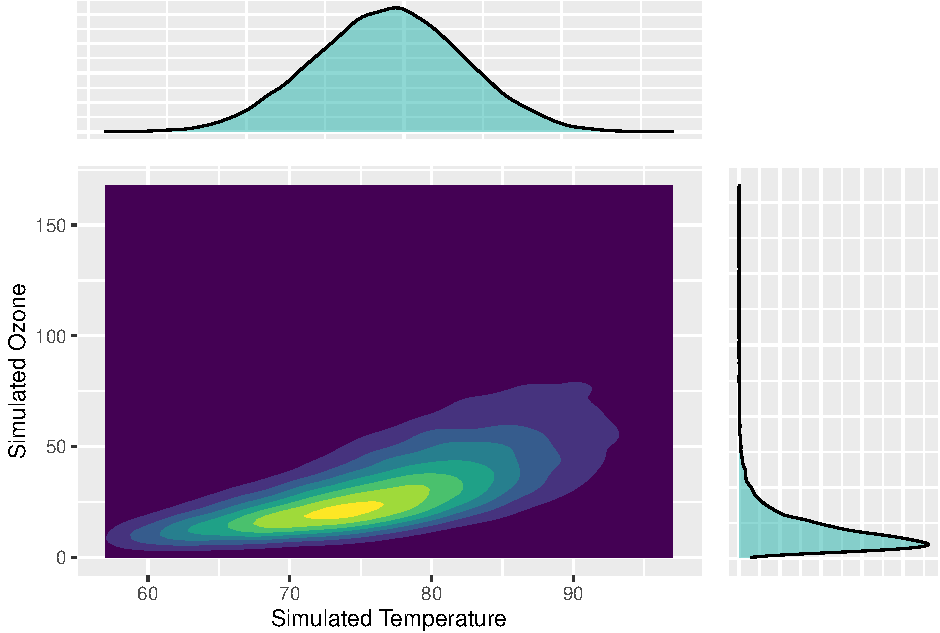
\includegraphics[width=0.85\linewidth]{article_bigsimr_files/figure-latex/ch030-plot-sim-1} 

}

\caption[Contour plot and marginal densities for the simulated bivariate distribution of Air Quality Temperatures and Ozone levels]{Contour plot and marginal densities for the simulated bivariate distribution of Air Quality Temperatures and Ozone levels. The simulated points mimic the observed data with respect to both the marginal characteristics and bivariate association.}\label{fig:ch030-plot-sim}
\end{figure}
\end{CodeChunk}

\hypertarget{simulations}{%
\section{Monte Carlo evaluations}\label{simulations}}

In this section, we conduct MC studies to investigate method
performance. Marginal parameter matching is straightforward in our
scheme as it is a sequence of univariate inverse probability transforms.
This process is both fast and exact. On the other hand, accurate and
computationally efficent dependency matching presents a challenge,
especially in the HD setting. To evaluate our methods in those respects,
we design the following numerical experiments to first assess accuracy
of matching dependency parameters in bivariate simulations and then time
the procedure in increasingly large dimension \(d\).

\hypertarget{bivariate-experiments}{%
\subsection{Bivariate experiments}\label{bivariate-experiments}}

We select bivariate simulation configurations to ultimately simulate our
motivating discrete-valued RNA-seq example. Thus, we proceed in
increasing departure from normality, leading to the multivariate
negative binomial (MVNB) model for our motivating data. We begin with
empirically evaluating the dependency matching across all three
supported correlations --- Pearson, Spearman, and Kendall --- in
identical, bivariate marginal configurations. For each pair of identical
margins, we vary the target correlation across \(\Omega\), the set of
possible admissible values for each correlation type, to evaluate the
simulation's ability to simulate all possible correlations. The
simulations progress from bivariate normal, to bivariate gamma
(non-normal yet continuous), and bivariate negative binomial (non-normal
and discrete).

Table @ref(tab:sims) lists our identical-marginal, bivariate simulation
configurations. We increase the simulate replicates \(B\) to visually
ensure that our results converge to the target correlations and gauge
efficiency. We select distributions beginning with a standard
multivariate normal (MVN) as we expect the performance to be exact (up
to MC error) for all correlation types. Then, we select a non-symmetric
continuous distribution: a standard (rate =1), two-component
multivariate gamma (MVG). Finally, we select distributions and marginal
parameter values that are motivated by our RNA-seq data, namely values
proximal to probabilities and sizes estimated from the data (see
\href{examples}{RNA-seq data application} for estimation details).
Specifically, we assume a MVNB with
\(p_1 = p_2 = 3\times10^{-4}, r_1 = r_2 = 4, \rho \in \Omega\).

For each of the unique 9 simulation configurations described above, we
estimate the correlation bounds and vary the correlations along a
sequence of 100 points evenly placed within the bounds, aiming to
explore \(\Omega\). Specifically, we set correlations
\(\{ \rho_1 = ( \hat{l} + \epsilon), \rho_2 = (\hat{l} + \epsilon) + \delta, \ldots, \rho_{100} = (\hat{u} - \epsilon) \}\),
with \(\hat{l}\) and \(\hat{u}\) being the estimated lower and upper
bounds, respectively, with increment value \(\delta\). The adjustment
factor, \(\epsilon=0.01\), is introduced to handle numeric issues when
the bound is specified exactly.

Figure @ref(fig:ch040-bPlot) displays the aggregated bivariate
simulation results. Table @ref(tab:ch040-BiError) contains the mean
absolute error (MAE) in reproducing the desired dependency measures for
the three bivariate scenarios.

\begin{CodeChunk}
\begin{table}

\caption{\label{tab:ch040-BiError}Average abolute error in matching the target dependency across the entire range of possible correlations for each bivariate marginal.}
\centering
\begin{tabular}[t]{lllr}
\toprule
No. of random vectors & Correlation type & Distribution & Mean abs. error\\
\midrule
1000 & Pearson & norm & 0.0156\\
1000 & Pearson & gamma & 0.0159\\
1000 & Pearson & nbinom & 0.0162\\
\addlinespace
1000 & Spearman & norm & 0.0175\\
1000 & Spearman & gamma & 0.0182\\
1000 & Spearman & nbinom & 0.0151\\
\addlinespace
1000 & Kendall & norm & 0.0130\\
1000 & Kendall & gamma & 0.0115\\
1000 & Kendall & nbinom & 0.0126\\
\addlinespace
10000 & Pearson & norm & 0.0060\\
10000 & Pearson & gamma & 0.0058\\
10000 & Pearson & nbinom & 0.0058\\
\addlinespace
10000 & Spearman & norm & 0.0062\\
10000 & Spearman & gamma & 0.0056\\
10000 & Spearman & nbinom & 0.0049\\
\addlinespace
10000 & Kendall & norm & 0.0033\\
10000 & Kendall & gamma & 0.0038\\
10000 & Kendall & nbinom & 0.0033\\
\addlinespace
1e+05 & Pearson & norm & 0.0018\\
1e+05 & Pearson & gamma & 0.0017\\
1e+05 & Pearson & nbinom & 0.0030\\
\addlinespace
1e+05 & Spearman & norm & 0.0017\\
1e+05 & Spearman & gamma & 0.0016\\
1e+05 & Spearman & nbinom & 0.0015\\
\addlinespace
1e+05 & Kendall & norm & 0.0010\\
1e+05 & Kendall & gamma & 0.0011\\
1e+05 & Kendall & nbinom & 0.0012\\
\bottomrule
\end{tabular}
\end{table}

\end{CodeChunk}

Overall, the studies show that our methodology is generally accurate
across the entire range of possible correlation for all three dependency
measures. Our Pearson matching performs nearly as well as Spearman or
Kendall, except for a slight increase in error for negative binomial
case.

\begin{CodeChunk}
\begin{figure}

{\centering 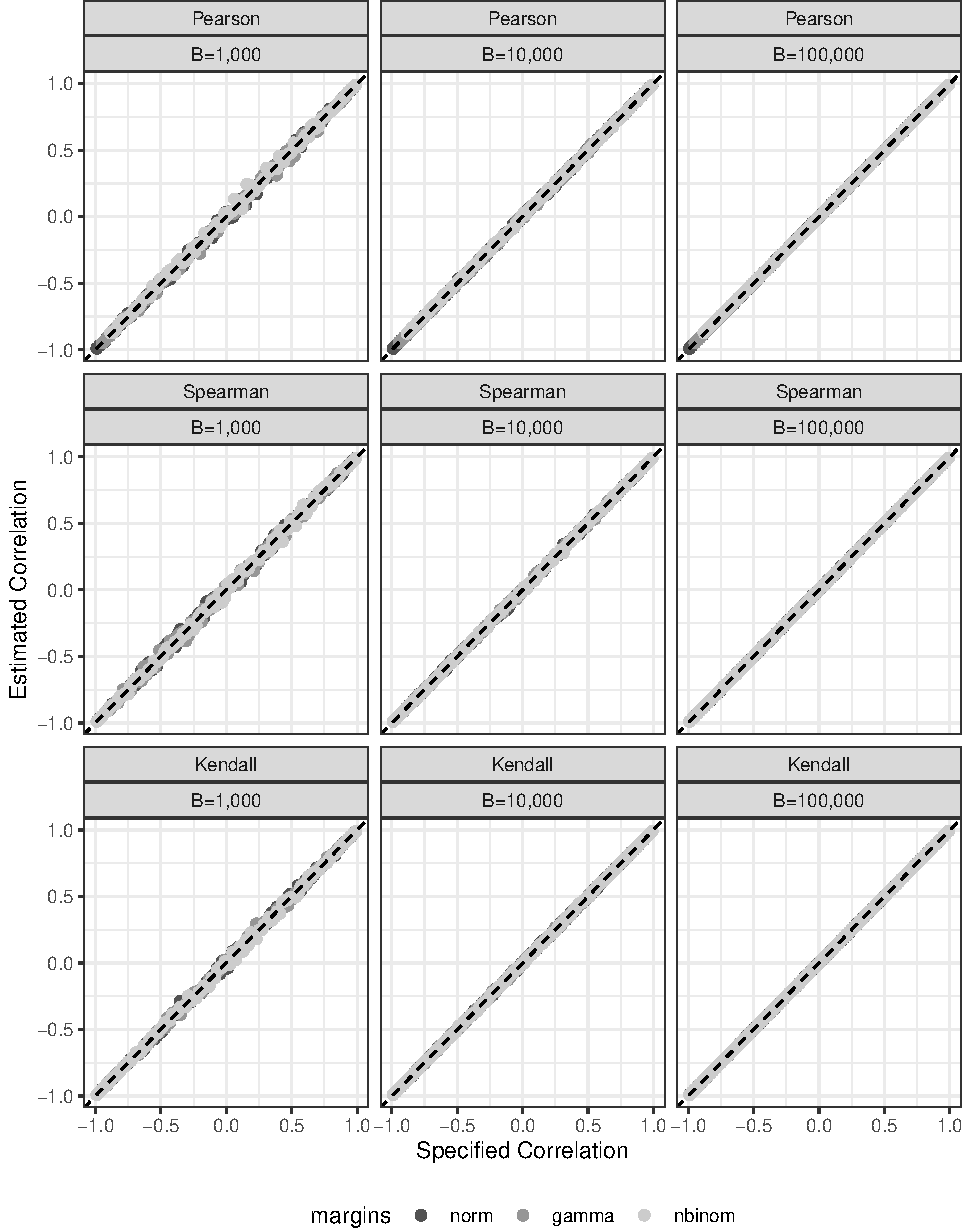
\includegraphics[width=0.85\linewidth]{article_bigsimr_files/figure-latex/ch040-bPlot-1} 

}

\caption[Bivariate simulations match target correlations across the entire range of feasible correlations]{Bivariate simulations match target correlations across the entire range of feasible correlations. The horizontal axis plots the specified target correlations for each bivariate margin. Normal margins are plotted in dark dark grey, gamma in medium grey, and negative binomial in light grey. As the number of simulated vectors $B$ increases from left to right, the variation in estimated correlations (vertical axis) decreases. The dashed line indicates equality between the specified and estimated correlations.}\label{fig:ch040-bPlot}
\end{figure}
\end{CodeChunk}

\hypertarget{scale-up-to-high-dimensions}{%
\subsection{Scale up to High
Dimensions}\label{scale-up-to-high-dimensions}}

With information of our method's accuracy from a low-dimensional
perspective, we now assess whether \texttt{bigsimr} can scale to larger
dimensional problems with practical computation times. We ultimately
generate \(B=1,000\) random vectors for
\(d=\{100, 250, 500, 1000, 2500, 5000, 10000\}\) for each correlation
type, \{Pearson, Spearman, Kendall\} while timing the algorithm's major
steps.

We first produce a synthetic ``data set'' by completing the following
steps:

\setstretch{1.5}

\begin{enumerate}
\def\labelenumi{\arabic{enumi}.}
\tightlist
\item
  Produce heterogeneous gamma marginals by randomly selecting the
  \(j^{th}\) gamma shape parameter from
  \(U_j \sim uniform(1,10), j=1,\ldots,d\) and the \(j^{th}\) rate
  parameter from \(V_j \sim exp(1/5), j=1,\ldots,d\), with the constant
  parameters determined arbitrarily.
\item
  Produce a random full-rank Pearson correlation matrix via
  \texttt{cor\_randPD} of size \(d \times d\).
\item
  Simulate a ``data set'' of \(1,000 \times d\) random vectors via
  \texttt{rvec}. \setstretch{2.0}
\end{enumerate}

With the synthetic data set in hand, we complete and time the following
four steps involved in a typical workflow (including correlation
estimation).

\setstretch{1.5}

\begin{enumerate}
\def\labelenumi{\arabic{enumi}.}
\tightlist
\item
  Estimate the correlation matrix from the ``data'' in the \emph{Compute
  Correlation} step.
\item
  Map the correlations to initialize the algorithm (Pearson to Pearson,
  Spearman to Pearson, or Kendall to Pearson) in the \emph{Adjust
  Correlation} step.
\item
  Check whether the mapping produces a valid correlation matrix and, if
  not, find the nearest PD correlation matrix in the \emph{Check
  Admissibility} step.
\item
  Simulate \(1,000\) vectors in the \emph{Simulate Data} step.
  \setstretch{2.0}
\end{enumerate}

The experiments are conducted on a MacBook Pro carrying a 2.4 GHz 8-Core
Intel Core i9 processor, with all 16 threads employed during
computation. Table @ref(tab:ch040-moderateDtab) displays the total
computation time for moderate dimesions (\(d \leq 500\)). In every
simullation setting, the 1,000 vectors are generated rapidly, executing
in under 2 seconds.

\begin{CodeChunk}
\begin{table}

\caption{\label{tab:tab:ch040-moderateDtab}Total time to produce 1,000 random vectors with a random correlation matrix and hetereogeneous gamma margins.}
\centering
\begin{tabular}[t]{llr}
\toprule
Dimension & Correlation type & Total Time (Seconds)\\
\midrule
100 & Pearson & 0.081\\
100 & Spearman & 0.027\\
100 & Kendall & 0.075\\
\addlinespace
250 & Pearson & 0.378\\
250 & Spearman & 0.062\\
250 & Kendall & 0.375\\
\addlinespace
500 & Pearson & 1.425\\
500 & Spearman & 0.135\\
500 & Kendall & 1.495\\
\bottomrule
\end{tabular}
\end{table}

\end{CodeChunk}

The results for \(d > 500\) show scalability to ultra-high dimensions
for all three correlation types, although the total times do become much
larger. Figure @ref(fig:ch040-largeDfig) displays computation times for
\(d=\{1000, 2500, 5000, 10000\}\). For \(d\) equal to 1000 and 2500, the
total time is under a couple of minutes. At \(d\) of 5000 and 10,000,
Pearson correlation matching in the \emph{Adjust Correlation} step
becomes costly. Interestingly, Pearson is actually faster than Kendall
for \(d=10,000\) due to bottlenecks in \emph{Compute Correlation} and
\emph{Check Admissibility}. Uniformly, matching Spearman correlations is
faster, with total times under 5 minutes for \(d=10,000\), making
Spearman the most computationally-friendly dependency type for our
package. With this in mind, we scaled the simulation to \(d=20,000\) for
the Spearman type and obtained the 1,000 vectors in under an hour (data
not shown). In principle, this would enable the simulation of an entire
human-derived RNA-seq data set. We note that for a given target
correlation matrix and margins, steps 1, 2, and 3 only need to be
computed once and the fourth step, \emph{Simulate Data}, is nearly
instaneous for all settings considered.

\begin{CodeChunk}
\begin{figure}

{\centering 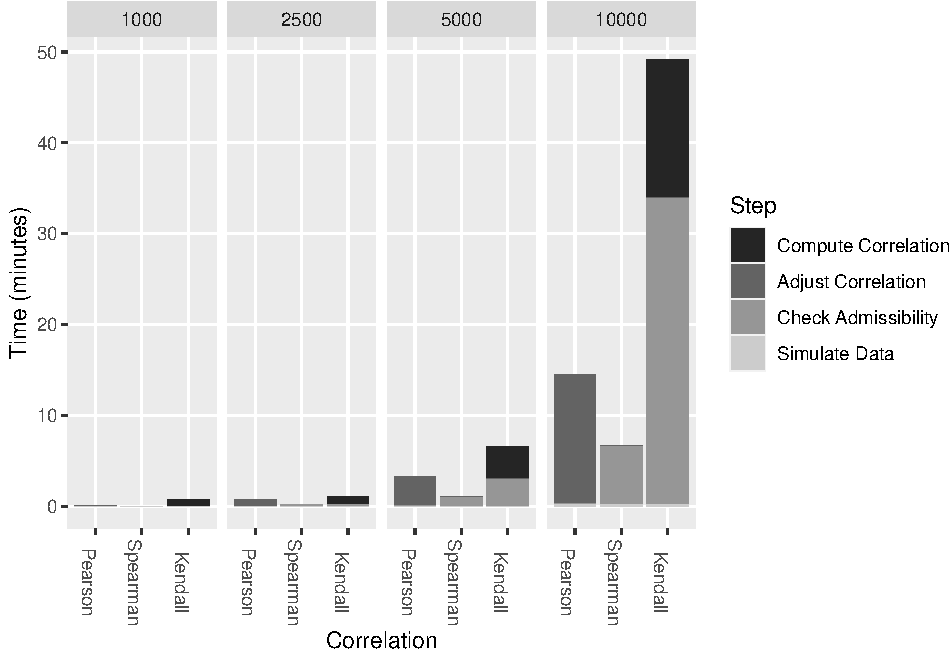
\includegraphics[width=0.85\linewidth]{article_bigsimr_files/figure-latex/ch040-largeDfig-1} 

}

\caption[Computation times for HD multivariate gamma simulation]{Computation times for HD multivariate gamma simulation.}\label{fig:ch040-largeDfig}
\end{figure}
\end{CodeChunk}

\emph{Limitations, conclusions, and recommendations}

In the bivariate studies, we chose arbitrary simulation parameters for
three distributions, moving from the Gaussian to discrete and non-normal
MVNB. Under these conditions, the simulated random vectors sample the
desired bivariate distribution across the entire range of pairwise
correlations for the three dependency measures. The simulation results
could differ for other choices of simulation settings. Specifying
extreme correlations near the boundary or Frechet bounds could result in
poor simulation performance. Fortunately, it is straightforward to
evaluate simulation performance by using strategies similar to those
completed above. We expect our random vector generation to perform well
for the vast majority of NORTA-feasible correlation matrices, but advise
to check the performance before making inferences/further analyses.

Somewhat surprising, Kendall estimation and nearest PD computation scale
poorly compared to Spearman and, even, approximate Pearson matching. In
our experience, Kendall computation times are sensitive to the number of
cores, benefiting from multi-core parallelization. This could mitigate
some of the current algorithmic/implementation shortcomings. Despite
this, Kendall matching is still feasible for most HD data sets. Finally,
we note that one could use our single-pass algorithm
\texttt{cor\_fastPD} to produce a `close' (not nearest PD) to scale to
even higher dimensions with some loss of accuracy.

\hypertarget{examples}{%
\section{RNA-seq data application}\label{examples}}

This section demonstrates how to simulate multivariate data using
\texttt{bigsimr}, aiming to replicate the structure of HD dependent
count data. In an illustration of our proposed methodology, we seek to
simulate RNA-sequencing data by producing simulated random vectors
mimicking the observed data and its generating process. Modeling RNA-seq
using multivariate probability distributions is natural as inter-gene
correlation occurs during biological processes \citep{Wang2009b}. And
yet, many models do not account for this, leading to major disruptions
to the operating characteristics of statistical estimation, testing, and
prediction. See \citet{Efron2012} for a detailed discussion with related
methods and \citet{Wu2012b}, \citet{Schissler2018};
\citet{Schissler2019} for applied examples. The following subsections
apply \texttt{bigsimr}'s methods to real RNA-seq data, including
replicating an estimated parametric structure, probability estimation,
and evaluation of correlation estimation efficiency.

\hypertarget{simulating-high-dimensional-rna-seq-data}{%
\subsection{Simulating High-Dimensional RNA-seq
data}\label{simulating-high-dimensional-rna-seq-data}}

We begin by estimating the structure of the TCGA BRCA RNA-seq data set.
Ultimately, we will simulate \(B=10,000\) random vectors
\({\bf Y}=(Y_1, \ldots, Y_d)^\top\) with \(d=1000\). We assume a MVNB
model as RNA-seq counts are often over-dispersed and correlated. Since
all \(d\) selected genes exhibit over-dispersion (data not shown), we
proceed to estimate the NB parameters \((r_i, p_i), i=1,\ldots,d\), to
determine the target marginal PMFs \(f_i\). To complete specification of
the simulation algorithm inputs, we estimate the Spearman correlation
matrix \(R_S\) to characterize dependency.

With this goal in mind, we first estimate the desired correlation matrix
using the fast implementation provided by \texttt{bigsimr}:

\begin{CodeChunk}
\begin{CodeInput}
R> # Estimate Spearman's correlation on the count data
R> R_S <- bs$cor(as.matrix(brca1000), bs$Spearman)
\end{CodeInput}
\end{CodeChunk}

Next, we estimate the marginal parameters. We use method of moments to
estimate the marginal parameters for the multivariate negative binomial
model. The marginal distributions are from the same probability family
(NB), yet they are heterogeneous in terms of the parameters probability
and size \((p_i, n_i)\) for \(i,\ldots,d\). The functions below support
this estimation for later use in \texttt{rvec}.

\begin{CodeChunk}
\begin{CodeInput}
R> make_nbinom_margins <- function(sizes, probs) {
+   margins <- lapply(1:length(sizes), function(i) {
+     dist$NegativeBinomial(sizes[i], probs[i])
+   })
+   do.call(c, margins)
+ }
\end{CodeInput}
\end{CodeChunk}

We apply these estimators to the highest-expressing 1000 genes across
the 878 patients:

\begin{CodeChunk}
\begin{CodeInput}
R> nbinom_fit <- apply(brca1000, 2, mom_nbinom)
R> sizes <- nbinom_fit["size",]
R> probs <- nbinom_fit["prob",]
R> nb_margins <- make_nbinom_margins(sizes, probs)
\end{CodeInput}
\end{CodeChunk}

Notably, the estimated marginal NB probabilities \(\{ \hat{p}_i \}\) are
small --- ranging in the interval
\([\ensuremath{7.5305\times 10^{-7}} , \ensuremath{5.6592\times 10^{-4}}]\).
This gives rise to highly variable counts and, thus, less restriction on
potential pairwise correlation pairs. Given the marginals, we now
specify targets and check admissibility of the specified correlation
matrix.

\begin{CodeChunk}
\begin{CodeInput}
R> # 1. Mapping step first
R> R_X <- bs$cor_convert(R_S, bs$Spearman, bs$Pearson)
R> # 2a. Check admissibility
R> (is_valid_corr <- bs$iscorrelation(R_X))
\end{CodeInput}
\begin{CodeOutput}
[1] FALSE
\end{CodeOutput}
\begin{CodeInput}
R> # 2b. compute nearest correlation
R> if (!is_valid_corr) {
+   R_X_pd <- bs$cor_nearPD(R_X)
+   ## Quantify the error
+   targets      <- R_X[lower.tri(R_X, diag = FALSE)]
+   approximates <- R_X_pd[lower.tri(R_X_pd, diag = FALSE)]
+   R_X          <- R_X_pd
+ }
R> summary(abs(targets - approximates))
\end{CodeInput}
\begin{CodeOutput}
    Min.  1st Qu.   Median     Mean  3rd Qu.     Max. 
0.000000 0.000201 0.000432 0.000534 0.000753 0.006931 
\end{CodeOutput}
\end{CodeChunk}

As seen above \(R_X\) is not strictly admissible in our scheme (as seen
by the non-positive definite result above). However, the approximation
is close with a maximum absolute error of 0.0069 and average absolute
error of \ensuremath{5.3366\times 10^{-4}} across the
\ensuremath{4.995\times 10^{5}} correlations. With the inputs
configured, \texttt{rvec} is executed to produce a synthetic RNA-seq
data set:

\begin{CodeChunk}
\begin{CodeInput}
R> sim_nbinom <- bs$rvec(10000, R_X, nb_margins) 
\end{CodeInput}
\end{CodeChunk}

Figure @ref(fig:ch050-simDataFig) displays the simulated counts and
pairwise relationships for our example genes from Table
@ref(tab:ch010-realDataTab). Simulated counts roughly mimic the observed
data but with a smoother appearance due to the assumed parametric form
and with less extreme points then the observed data in Figure
@ref(fig:ch010-realDataFig). Figure @ref(fig:ch050-figBRCA) compares the
specified target parameter (horizontal axis) with the corresponding
quantities estimated from the simulated data (vertical axis). The
evaluation shows that the simulated counts approximately match the
target parameters and exhibit the full range of estimated correlations
from the data.

\begin{CodeChunk}
\begin{figure}

{\centering 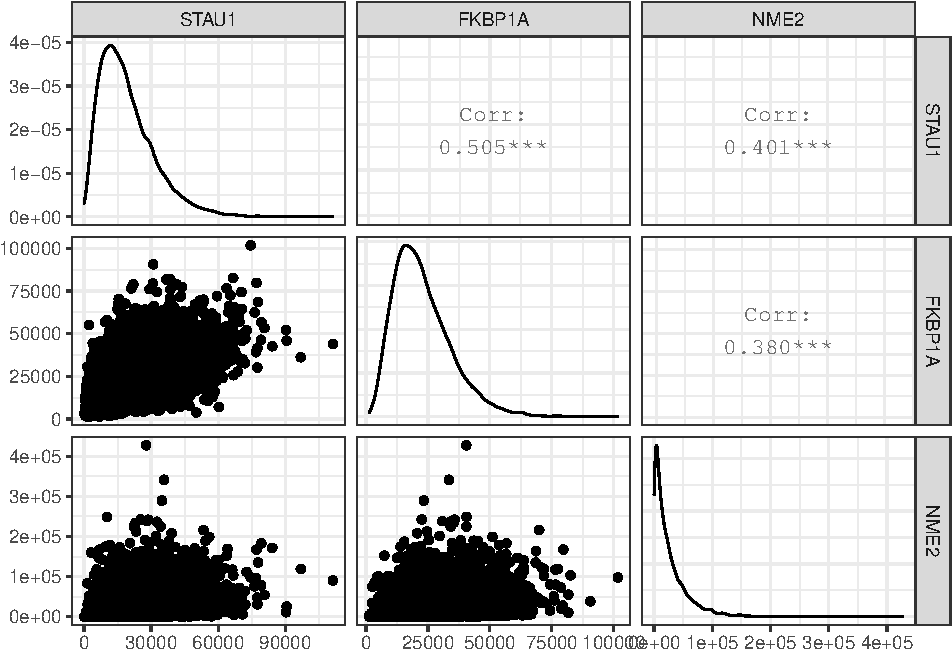
\includegraphics[width=0.85\linewidth]{article_bigsimr_files/figure-latex/ch050-simDataFig-1} 

}

\caption[Simulated data for three selected high-expressing genes generally replicates the estimated data structure]{Simulated data for three selected high-expressing genes generally replicates the estimated data structure. The data do not exhibit outlying points, but do possess the desired Spearman correlations, central tendencies, and discrete values.}\label{fig:ch050-simDataFig}
\end{figure}
\end{CodeChunk}

\begin{CodeChunk}
\begin{figure}

{\centering 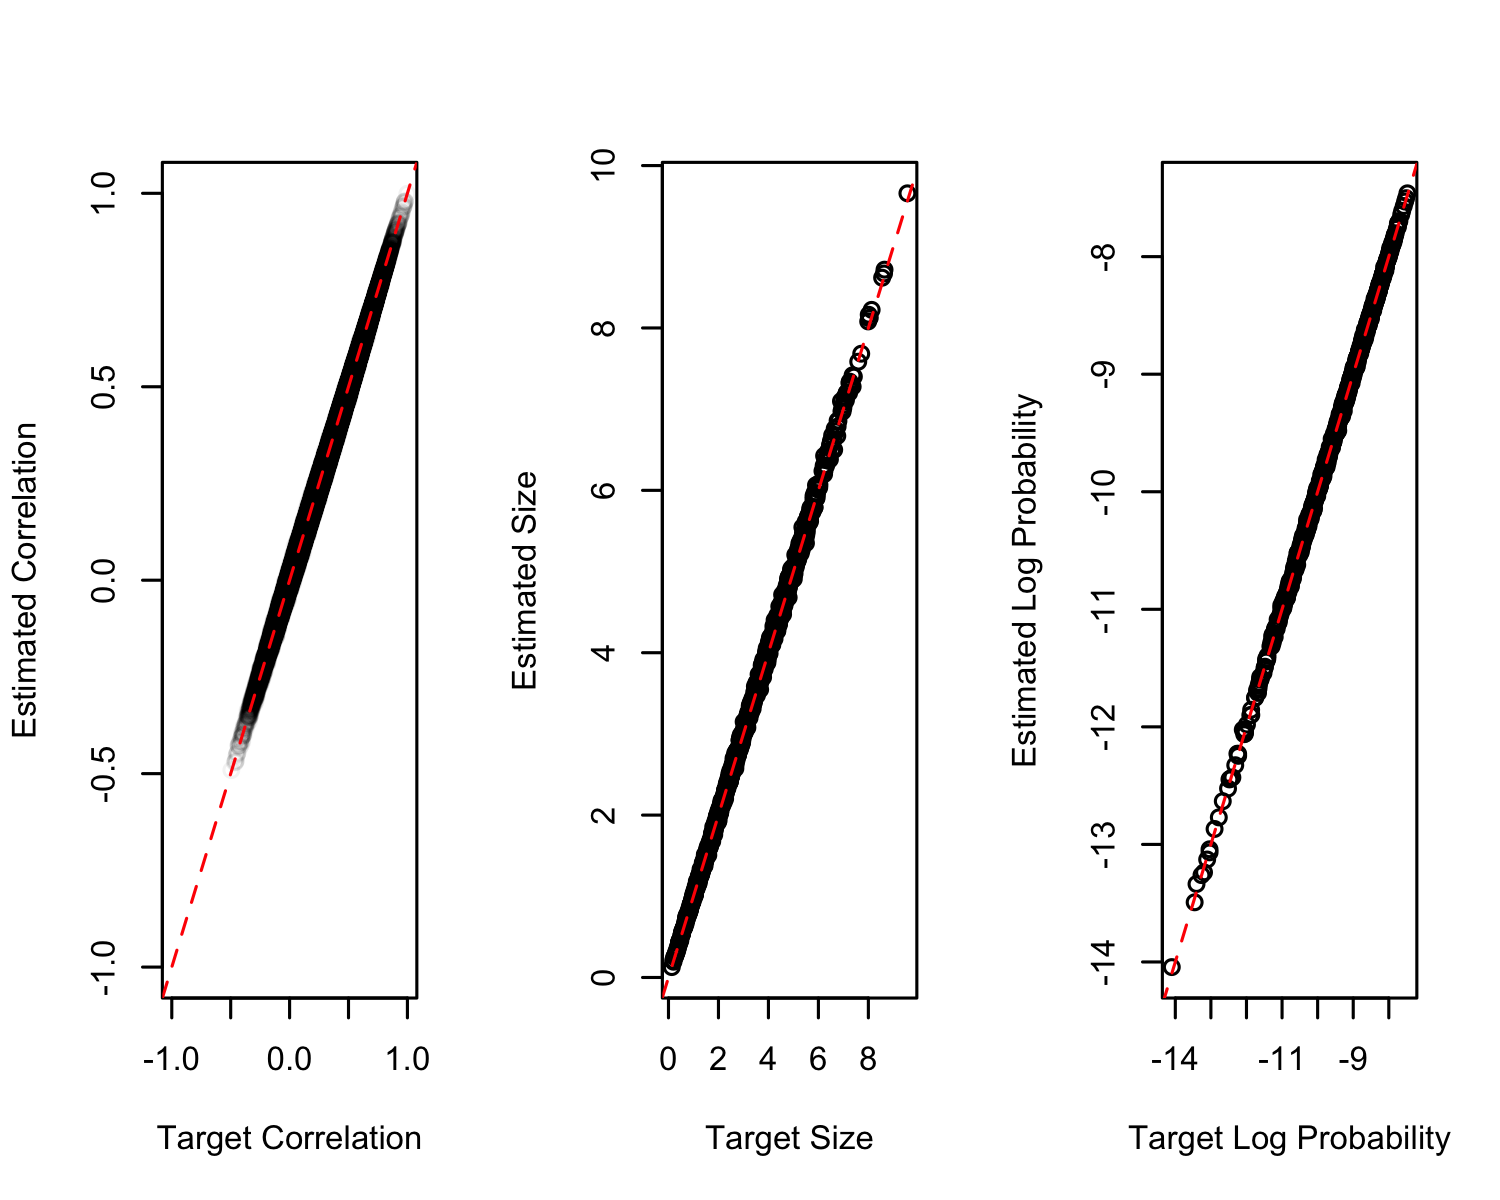
\includegraphics[width=0.8\linewidth]{fig/ch050-figBRCA} 

}

\caption[Simulated random vectors from a multivariate negative binomial replicate the estimated structure from an RNA-seq data set]{Simulated random vectors from a multivariate negative binomial replicate the estimated structure from an RNA-seq data set. The dashed red lines indicate equality between estimated parameters from simulated data (vertical axes) and the specified target parameters (horizontal axes).}\label{fig:ch050-figBRCA}
\end{figure}
\end{CodeChunk}

\emph{Limitations, conclusions, and recommendations}

The results show overall aquedate simulation performance for our choice
of parameters settings. Our settings were motivated by modeling
high-expressing genes from the TCGA BRCA data set. In general, the
ability to match marginal and dependence parameters depends on the
particular joint probability model. We recommend to evaluate and tune
your simulation until you can be assured of the accuracy.

\hypertarget{simulation-based-joint-probability-calculations}{%
\subsection{Simulation-based joint probability
calculations}\label{simulation-based-joint-probability-calculations}}

Many statistical tasks require evaluation of a joint probability mass
(or density) function:

\[
P( {\bf Y} = {\bf y} ), \: y_i \in \chi_i.
\]

where \(\chi_i\) is the sample space for the \(i^{th}\) component of the
random vector \(\bf{Y}\). Compact representations with convenient
computational forms are rare for high-dimensional constructions,
especially with heterogeneous marginal distributions. Given a large
number of simulated vectors as produced above, estimated probabilities
are readily given by counting the proportion of simulated vectors
meeting the desired condition. In our motivating application, one could
ask: what is the probability that all genes are expressed greater than a
certain threshold value \({\bf y}_0\)? This can be estimated as

\[
\hat{P}( {\bf Y} \ge {\bf y_0 } ) = \frac{1}{B} \sum_{b=1}^B I( {\bf Y}^{ (b) } \ge {\bf y_0} ),
\]

where \({\bf Y}^{(b)}\) is the \(b^{th}\) simulated vector from a total
of \(B\) simulation replicates and \(I(\cdot)\) is the indicator
function. For example, we can estimate from our \(B=10,000\) simulated
vectors that the probability of all genes expressing (i.e.,
\({\bf y}_i \geq 1, \forall \; i\)) is \(0.6015\).

\begin{CodeChunk}
\begin{CodeInput}
R> pHat
\end{CodeInput}
\begin{CodeOutput}
[1] 0.6015
\end{CodeOutput}
\end{CodeChunk}

\hypertarget{evaluation-of-correlation-estimation-efficiency}{%
\subsection{Evaluation of correlation estimation
efficiency}\label{evaluation-of-correlation-estimation-efficiency}}

To conclude the example applications, we demonstrate how
\texttt{bigsimr} can be used to evaluate correlation estimation
efficiency. In particular, we wish to assess the error in our
correlation estimation above. We used a conventional method, based on
classical statistical theory which was not designed for high-dimensional
data. Indeed, high-dimensional covariance estimation is an active area
of statistical science; see, for example, \citet{Won2013g} or
\citet{VanWieringen2016}.

In this small example, we simulate \(m=30\) data sets with the number of
simulated vectors matching the number of patients in the BRCA data set,
\(N=878\). At each iteration, we estimate the quadratic loss (residual
sum of squared errors) from the specified \({\bf R}_{S}\), producing a
distribution of loss values.

\begin{CodeChunk}
\begin{CodeInput}
R> # Simulate random vectors equal to the sample size
R> N <- nrow(example_brca)
R> # create m random vectors and estimate correlation
R> simRho <- replicate(n = m, expr = {
+   tmpSim <- bs$rvec(N , R_X, nb_margins)
+   bs$cor(tmpSim, bs$Spearman)
+ }, simplify = FALSE)
\end{CodeInput}
\end{CodeChunk}

The \texttt{R} summary function supplies the mean-augmented five-number
summary of the Frobenius loss from the target. This distribution could
be compared to bespoke HD covariance estimators for guidance on whether
the additional complexity and computation time are warranted.

\begin{CodeChunk}
\begin{CodeInput}
R> frobenius_loss <- sapply(simRho, function(R) norm( R - R_S, type = "F")  )
R> summary(frobenius_loss)
\end{CodeInput}
\begin{CodeOutput}
   Min. 1st Qu.  Median    Mean 3rd Qu.    Max. 
   26.0    28.5    31.2    31.4    32.9    43.0 
\end{CodeOutput}
\end{CodeChunk}

\hypertarget{discussion}{%
\section{Conclusion and discussion}\label{discussion}}

We developed a general-purpose high-dimensional multivariate simulation
algorithm and provide a user-friendly, high-performance \texttt{R}
package \texttt{bigsimr}, Julia package \texttt{Bigsimr} and Python
package \texttt{bigsimr}. The random vector generation method is
inspired by NORTA \citep{Cario1997} and Gaussian copula-based approaches
\citep[\citet{BF17}, \citet{Xia17}]{MB13}. The major contributions of
this work are methods and software for flexible, scalable simulation of
HD multivariate probability distributions with broad data analytic
applications for modern, big-data statistical computing. For example,
one could simulate high-resolution time series data, such as those
consistent with an auto-regressive moving average model exhibiting a
specified Spearman structure. Or our methods could be used to simulate
sparsely correlated data, as many HD methods assume, via specifying a
\emph{spiked correlation matrix}.

There are limitations to the methodology and implementation. We could
only investigate selected multivariate distributions in our Monte Carlo
studies. There may be instances that the methods do not perform well.
Along those lines, we expect that correlation values close to the
boundary of the feasible region could result in algorithm failure.
Another issue is that for discrete distributions, we use continuous
approximations when the support set is large. This could limit the
scalability/accuracy for particular discrete/mixed multivariate
distributions. Our method would also benefit computationally from faster
Kendall estimation and more finely tuned nearest PD calculation for
non-admissible Kendall matrices.

\newpage

\hypertarget{misc}{%
\section*{Supplementary Materials}\label{misc}}
\addcontentsline{toc}{section}{Supplementary Materials}

We provide an open-source implementation of our methodology as the
\texttt{Bigsimr.jl} Julia package, hosted on github at
\url{https://github.com/adknudson/Bigsimr.jl}. Additionally we provide R
and Python interfaces to \texttt{Bigsimr}, respectively at
\url{https://github.com/SchisslerGroup/r-bigsimr} and
\url{https://github.com/SchisslerGroup/python-bigsimr}.
\texttt{Bigsimr.jl} is an ongoing project, and feature requests or
issues can be submitted to
\url{https://github.com/adknudson/Bigsimr.jl/issues}.

\begin{CodeChunk}


\begin{center}
\includegraphics[width=0.05\linewidth]{images/hex-bigsimr} \end{center}

\end{CodeChunk}

\hypertarget{acknowledgments}{%
\section*{Acknowledgment(s)}\label{acknowledgments}}
\addcontentsline{toc}{section}{Acknowledgment(s)}

The authors gratefully acknowledge Heather Knudson's graphic design for
the \texttt{bigsimr} R Package. The results published here are in whole
or part based upon data generated by the TCGA Research Network:
\url{https://www.cancer.gov/tcga}.

\hypertarget{coi}{%
\section*{Disclosure statement}\label{coi}}
\addcontentsline{toc}{section}{Disclosure statement}

The authors report no conflict of interest.

\hypertarget{funding}{%
\section*{Funding}\label{funding}}
\addcontentsline{toc}{section}{Funding}

Research reported in this publication was supported by grants from the
National Institutes of General Medical Sciences (5 U54 GM104944,
GM103440) from the National Institutes of Health.

\newpage

\hypertarget{appendix}{%
\section*{Appendix}\label{appendix}}
\addcontentsline{toc}{section}{Appendix}

\noindent Consider a bivariate example where we have a correlated
\((Y_1, Y_2)^\top\) with \(Y_1\sim N(\mu_1, \sigma_1^2)\) (normal) and
\(Y_2\sim LN(\mu_2, \sigma_2^2)\) (lognormal). First, let us note that
when we get such a vector from the \texttt{bigsimr} package then in fact
it can be represented as

\begin{equation}
\label{eq:kram1}
(Y_1, Y_2)^\top \stackrel{d}{=} \left(X_1, e^{X_2}\right)^\top,
\end{equation}

where \((X_1, X_2)^\top \sim N_2(\boldsymbol \mu, \boldsymbol \Sigma)\),
which is bivariate normal with mean vector
\(\boldsymbol \mu = (\mu_1, \mu_2)^\top\) and variance-covariance matrix

\begin{equation}
\label{eq:kram2}
\boldsymbol \Sigma = 
\begin{bmatrix}
\sigma_1^2 & \rho \sigma_1\sigma_2\\
\rho \sigma_1\sigma_2 & \sigma_2^2
\end{bmatrix}
\end{equation}

To see this, consider the three steps of the NORTA construction:

\begin{enumerate}

\item Generate $(Z_1, Z_2)^\top \sim N_2(\boldsymbol 0, \boldsymbol R)$, where 

\begin{equation}
\label{eq:kram3}
\boldsymbol R = 
\left[
\begin{array}{cc}
1 & \rho \\
\rho & 1
\end{array}
\right].
\end{equation}


\item Transform $(Z_1, Z_2)^\top$ to $(U_1, U_2)^\top$ viz. $U_i =\Phi(Z_i)$,  $i=1,2$, where $\Phi(\cdot)$ is the standard normal CDF. 

\item Return $(Y_1, Y_2)^\top$, where $Y_i=F_i^{-1}(U_i)$, $i=1,2$, and $F_i(\cdot)$ is the CDF of $Y_i$ and $F_i^{-1}(\cdot)$ is its inverse (the quantile function). 

\end{enumerate}

In this example, \(F_1\) is the CDF of \(N(\mu_1, \sigma_1^2)\) while
\(F_2\) is the CDF of \(LN(\mu_2, \sigma_2^2)\), so that the two
required quantile functions are

\begin{equation}
\label{eq:kram4}
F_1^{-1}(u) = \mu_1+\sigma_1 \Phi^{-1}(u)\,\,\, \mbox{and} \,\,\, F_2^{-1}(u) = e^{\mu_2+\sigma_2 \Phi^{-1}(u)}, 
\end{equation}

as can be seen by standard calculation. Thus, when we apply Step 3 of
the NORTA algorithm, we get

\begin{equation}
\label{eq:kram5}
F_1^{-1}(U_1) = \mu_1+\sigma_1 \Phi^{-1}(\Phi(Z_1)) =  \mu_1+\sigma_1 Z_1 \,\,\, \mbox{and} \,\,\, F_2^{-1}(U_2) = e^{\mu_2+\sigma_2 \Phi^{-1}(\Phi(Z_2))} = e^{\mu_2+\sigma_2 Z_2}, 
\end{equation}

where
\((X_1, X_2)^\top = (\mu_1+\sigma_1 Z_1, \mu_2+\sigma_2 Z_2)^\top \sim N_2(\boldsymbol \mu, \boldsymbol \Sigma)\).
Consequently, the vector \((Y_1, Y_2)^\top\) obtained in Step 3 of the
algorithm has the structure provided by (\ref{eq:kram1}).

\vspace{0.1in}

\noindent Next, we provide the exact covariance structure of the random
vector \((Y_1, Y_2)^\top\) given by (\ref{eq:kram1}), and relate the
correlation of \(Y_1\) and \(Y_2\) to \(\rho\), which is the correlation
of the normal variables \(Z_1\), \(Z_2\) (and also \(X_1\) and \(X_2\)).
A straightforward albeit somewhat tedious algebra produces the following
result.

\begin{lemma}
Let ${\bf Y} = (Y_1, Y_2)^\top$ admit the stochastic representation (\ref{eq:kram1}), where ${\bf X} = (X_1, X_2)^\top \sim N_2(\boldsymbol \mu, \boldsymbol \Sigma)$ with $\boldsymbol \mu$ and $\boldsymbol \Sigma$ as above. Then the mean vector and the variance-covariance matrix of ${\bf Y}$ are given by 

\begin{equation}
\label{eq:kram6}
\boldsymbol \mu_{{\bf Y}} = \left(\mu_1, e^{\mu_2+\sigma_2^2/2}\right)^\top
\end{equation}

and 

\begin{equation}
\label{eq:kram7}
\boldsymbol \Sigma = 
\begin{bmatrix}
\sigma_1^2 & \rho \sigma_1\sigma_2  e^{\mu_2+\sigma_2^2/2}  \\
\rho \sigma_1\sigma_2 e^{\mu_2+\sigma_2^2/2} & \left[ e^{\mu_2+\sigma_2^2/2}\right]^2 \left[e^{\sigma_2^2} -1 \right],
\end{bmatrix}
\end{equation}

respectively. 
\end{lemma}

\begin{proof}
The values of the means and the variances are obtained immediately from normal marginal distribution of $Y_1$ and lognormal marginal distribution of $Y_2$. It remains to establish the covariance of $Y_1$ and $Y_2$, 

\begin{equation}
\label{eq:covy1y2}
\mbox{Cov}(Y_1, Y_2) = \mathbb E(Y_1 Y_2) - \mathbb E(Y_1)\mathbb E(Y_2), 
\end{equation}

and in particular the first expectation on the right-hand-side above. By using the tower property of expectations, the latter expectation can be expressed as 

\begin{equation}
\label{eq:kre1}
\mathbb E(Y_1 Y_2)  =  \mathbb E\left(X_1 e^{X_2}\right)  =  \mathbb E \left\{ \mathbb E \left(X_1 e^{X_2} | X_1 \right) \right\} = \mathbb E \left\{ X_1 \mathbb E \left(e^{X_2} | X_1 \right) \right\}.
\end{equation}

Further, by using the fact that the conditional distribution of $X_2$ given $X_1=x_1$ is normal with mean $\mathbb E(X_2|X_1=x_1) = \mu_2+\rho\sigma_2(x_1-\mu_1)/\sigma_1$ and variance $\sigma_2^2(1-\rho^2)$, one can relate the inner expectation on the far right in (\ref{eq:kre1}) to the moment generating function $M(t)$ of this conditional distribution evaluated at $t=1$, leading to 

\begin{equation}
\label{eq:kre2}
E \left(e^{X_2} | X_1 \right) = e^{ \mu_2+\rho\sigma_2(x_1-\mu_1)/\sigma_1 + \sigma_2^2(1-\rho^2)/2},
\end{equation}

so that 

\begin{equation}
\label{eq:kre3}
\mathbb E(Y_1 Y_2)  =  e^{ \mu_2+ \frac{1}{2} \sigma_2^2(1-\rho^2)} \mathbb E \left\{ X_1 e^{ \rho\frac{\sigma_2}{\sigma_1} (X_1-\mu_1)} \right\}.
\end{equation}

Since $X_1$ is normal with mean $\mu_1$ and variance $\sigma_1^2$, the expectation in (\ref{eq:kre3}) becomes 

\begin{equation}
\label{eq:kre4}
\mathbb E \left\{ X_1 e^{ \rho\frac{\sigma_2}{\sigma_1} (X_1-\mu_1)} \right\} = \int_{-\infty}^\infty x_1 e^{ \rho\frac{\sigma_2}{\sigma_1} (x_1-\mu_1)} \frac{1}{\sqrt{2\pi}\sigma_1} e^{-\frac{1}{2\sigma_1^2}(x_1-\mu_1)^2}.
\end{equation}

Upon substituting $u=x_1-\mu_1$, followed by some algebra, we arrive at 

\begin{equation}
\label{eq:kre5}
\mathbb E \left\{ X_1 e^{ \rho\frac{\sigma_2}{\sigma_1} (X_1-\mu_1)} \right\} = e^{\frac{1}{2}\sigma_2^2\rho^2} \int_{-\infty}^\infty (u+\mu_1)  \frac{1}{\sqrt{2\pi}\sigma_1} e^{-\frac{1}{2\sigma_1^2}(u-\rho\sigma_1\sigma_2)^2}.
\end{equation}

Since the integral in (\ref{eq:kre5}) is the expectation $\mathbb E(X+\mu_1)$, where $X$ is normal with mean $\rho\sigma_1\sigma_2$ and variance $\sigma_1^2$, we conclude that 

\begin{equation}
\label{eq:kre6}
\mathbb E \left\{ X_1 e^{ \rho\frac{\sigma_2}{\sigma_1} (X_1-\mu_1)} \right\} = e^{\frac{1}{2}\sigma_2^2\rho^2} (\rho\sigma_1\sigma_2 +\mu_1),
\end{equation}

which, in view of (\ref{eq:kre3}), leads to 

\begin{equation}
\label{eq:kre7}
\mathbb E (Y_1Y_2) = e^{\mu_2 + \frac{1}{2}\sigma_2^2} (\rho\sigma_1\sigma_2 +\mu_1).
\end{equation}

Finally, (\ref{eq:covy1y2}), along with the expressions for the means of $Y_1$ and $Y_2$, produce the covariance of $Y_1$ and $Y_2$:

\begin{equation}
\label{eq:kre8}
\mbox{Cov}(Y_1, Y_2) = e^{\mu_2 + \frac{1}{2}\sigma_2^2} (\rho\sigma_1\sigma_2 +\mu_1) - \mu_1 e^{\mu_2 + \frac{1}{2}\sigma_2^2} = \rho\sigma_1\sigma_2 e^{\mu_2 + \frac{1}{2}\sigma_2^2}.
\end{equation}

This concludes the proof
\end{proof}

Using the above result, we can directly relate the correlation
coefficient of \(Y_1\) and \(Y_2\) with that of \(X_1\) and \(X_2\),

\begin{equation}
\label{eq:kram8}
\rho_{Y_1, Y_2} = \rho \frac{\sigma_2}{\sqrt{e^{\sigma_2^2} -1}},
\end{equation}

where \(\rho\) is the correlation of \(X_1\) and \(X_2\). The above
result is useful when studying the possible range of correlation of
\(Y_1\) and \(Y_2\) in the above example. It can be shown that the
factor on the far right in (\ref{eq:kram8}) is a monotonically
decreasing function of \(\sigma_2\) on \((0,\infty)\), with the limits
of 1 and 0 at zero and infinity, respectively. Thus, in principle, the
range of correlation of \(Y_1\) and \(Y_2\) is the same as that of
\(X_1\) and \(X_2\), as the factor on the far right in (\ref{eq:kram8})
can be made arbitrarily close to 1. However, by changing this factor we
may affect the marginal distributions of \(Y_1\) and \(Y_2\). It can be
shown that if the marginal distributions of \(Y_1\) and \(Y_2\) are
fixed, then the relation (\ref{eq:kram8}) becomes

\begin{equation}
\label{eq:kram9}
\rho_{Y_1, Y_2} = \rho \sqrt{\frac{\log(1+c_2^2)}{c_2^2}},
\end{equation}

where \(c_2=\sigma_{Y_2}/\mu_{Y_2}\) is the \emph{coefficient of
variation} (CV) of the variable \(Y_2\). Thus, the range of possible
correlations in this model is not affected by the distribution of
\(Y_1\), and is determined by the CV of \(Y_2\) as follows:

\begin{equation}
\label{eq:kram10}
- \sqrt{\frac{\log(1+c_2^2)}{c_2^2}} \leq \rho_{Y_1, Y_2} \leq \sqrt{\frac{\log(1+c_2^2)}{c_2^2}}. 
\end{equation}

Plugging in the estimates of these quantities from Section
@ref(package), we see that

\begin{equation}
\label{eq:kram11}
\frac{\hat{\sigma}_2}{\sqrt{e^{\hat{\sigma}_2^2} -1}} = 0.881.
\end{equation}

Thus, the possible range of correlation becomes \((-0.881, 0.881)\).
This agrees with the MC results provided.

\setstretch{1.0}

\bibliography{bigsimr.bib,packages.bib,alex.bib}


\end{document}
